Similar are results for the third case, the first problem without a classical solution. Without additional gradient penalty the method did not work well. For an example we show the all converged iteration steps for polynomial degree $k=2, k_{DH}=2$ in the table \ref{tab: l2 errors test 3}
\begin{table}[H]
%	\begin{subtable}[b]{0.45\textwidth}
		\centering
		\pgfplotstabletypeset[
		columns={iterations, l2error, h1error,N},
		    every row 0 column 0/.style={set content=init},
		]{\MAThreedegTwoTwo}
    	\caption{Error for $k=2, k_{DH}=2$}
%   \end{subtable}
%   ~
%	\begin{subtable}[b]{0.45\textwidth}
%		\centering
%%		\pgfplotstabletypeset[columns={iterations, l2error, h1error,N},
%%		    every row 0 column 0/.style={set content=init},
%%		]{\MAThreedegThreeThree}
%	\caption{Error for $k=3, k_{DH}=3$}
%	\end{subtable}
	\caption{Errors for test case \ref{test singularity}}
	\label{tab: l2 errors test 3}
\end{table}

The corresponding method with additional jump penalisation performed better and its results can be found in Figure \ref{fig: l2 errors test 3 jump} and \ref{fig: l2 errors test 3 jump}, as well as in Table \ref{tab: l2 errors test 3 jump}. 

As we can see the method with higher polynomial degree performs better albeit for $k=3$ Newton's method do not converge on the provided initial guess on a grid with $h=1/2$. The calculated numerical orders of table \ref{tab: order jump 3} show that measuring in the $H^1$ norm quadratic polynomials induce a twice as big convergence order than piecewise affine ansatz functions. Yet the data to calculate the numerical order provided only 5 points in the case $k=2$ and the error did not decrease very steadily.

\begin{figure}[H]
	\centering
	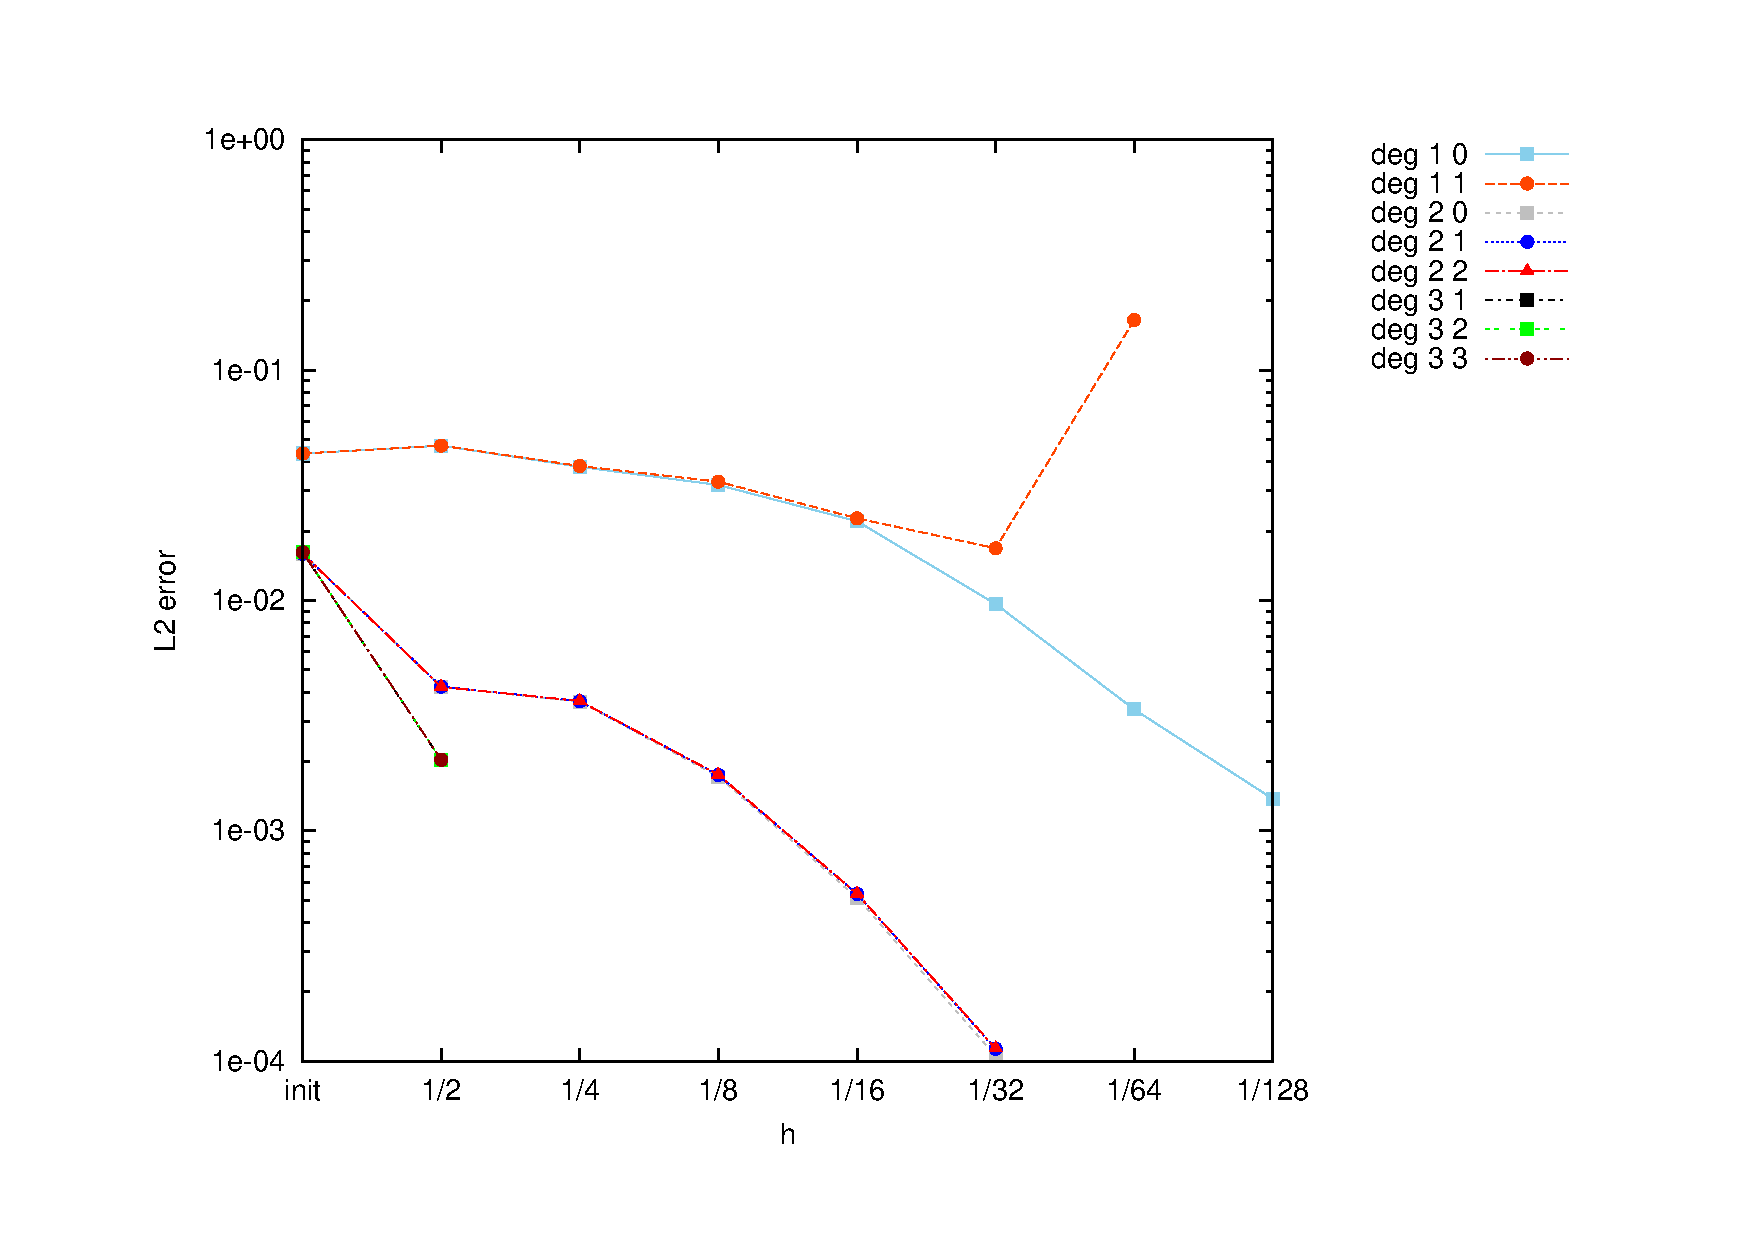
\includegraphics[scale =0.45]{../../FEniCS/diagrams/MA3_Neilan_GradJump_l2.pdf}
	\caption{$L^2$ errors for test case \ref{test singularity} and additional gradient jump penalty}
	\label{fig: l2 errors test 3 jump}
\end{figure}

\begin{table}[h]
	\begin{subtable}[b]{0.45\textwidth}
		\centering
		\pgfplotstabletypeset[columns={iterations, l2error, h1error,N},
		every row 0 column 0/.style={set content=init},
		]{\MAThreeJumpdegOneZero}
		\caption{Error for $k=1, k_{DH}=0$}
	\end{subtable}
	~
	\begin{subtable}[b]{0.45\textwidth}
		\centering
		\pgfplotstabletypeset[
		columns={iterations, l2error, h1error,N},
		every row 0 column 0/.style={set content=init},
		]{\MAThreeJumpdegTwoTwo}
		\caption{Error for $k=2, k_{DH}=2$}
	\end{subtable}
	\caption{Errors for test case \ref{test singularity} and additional gradient jump penalty}
	\label{tab: l2 errors test 3 jump}
\end{table}	
\begin{figure}[H]
	\centering
	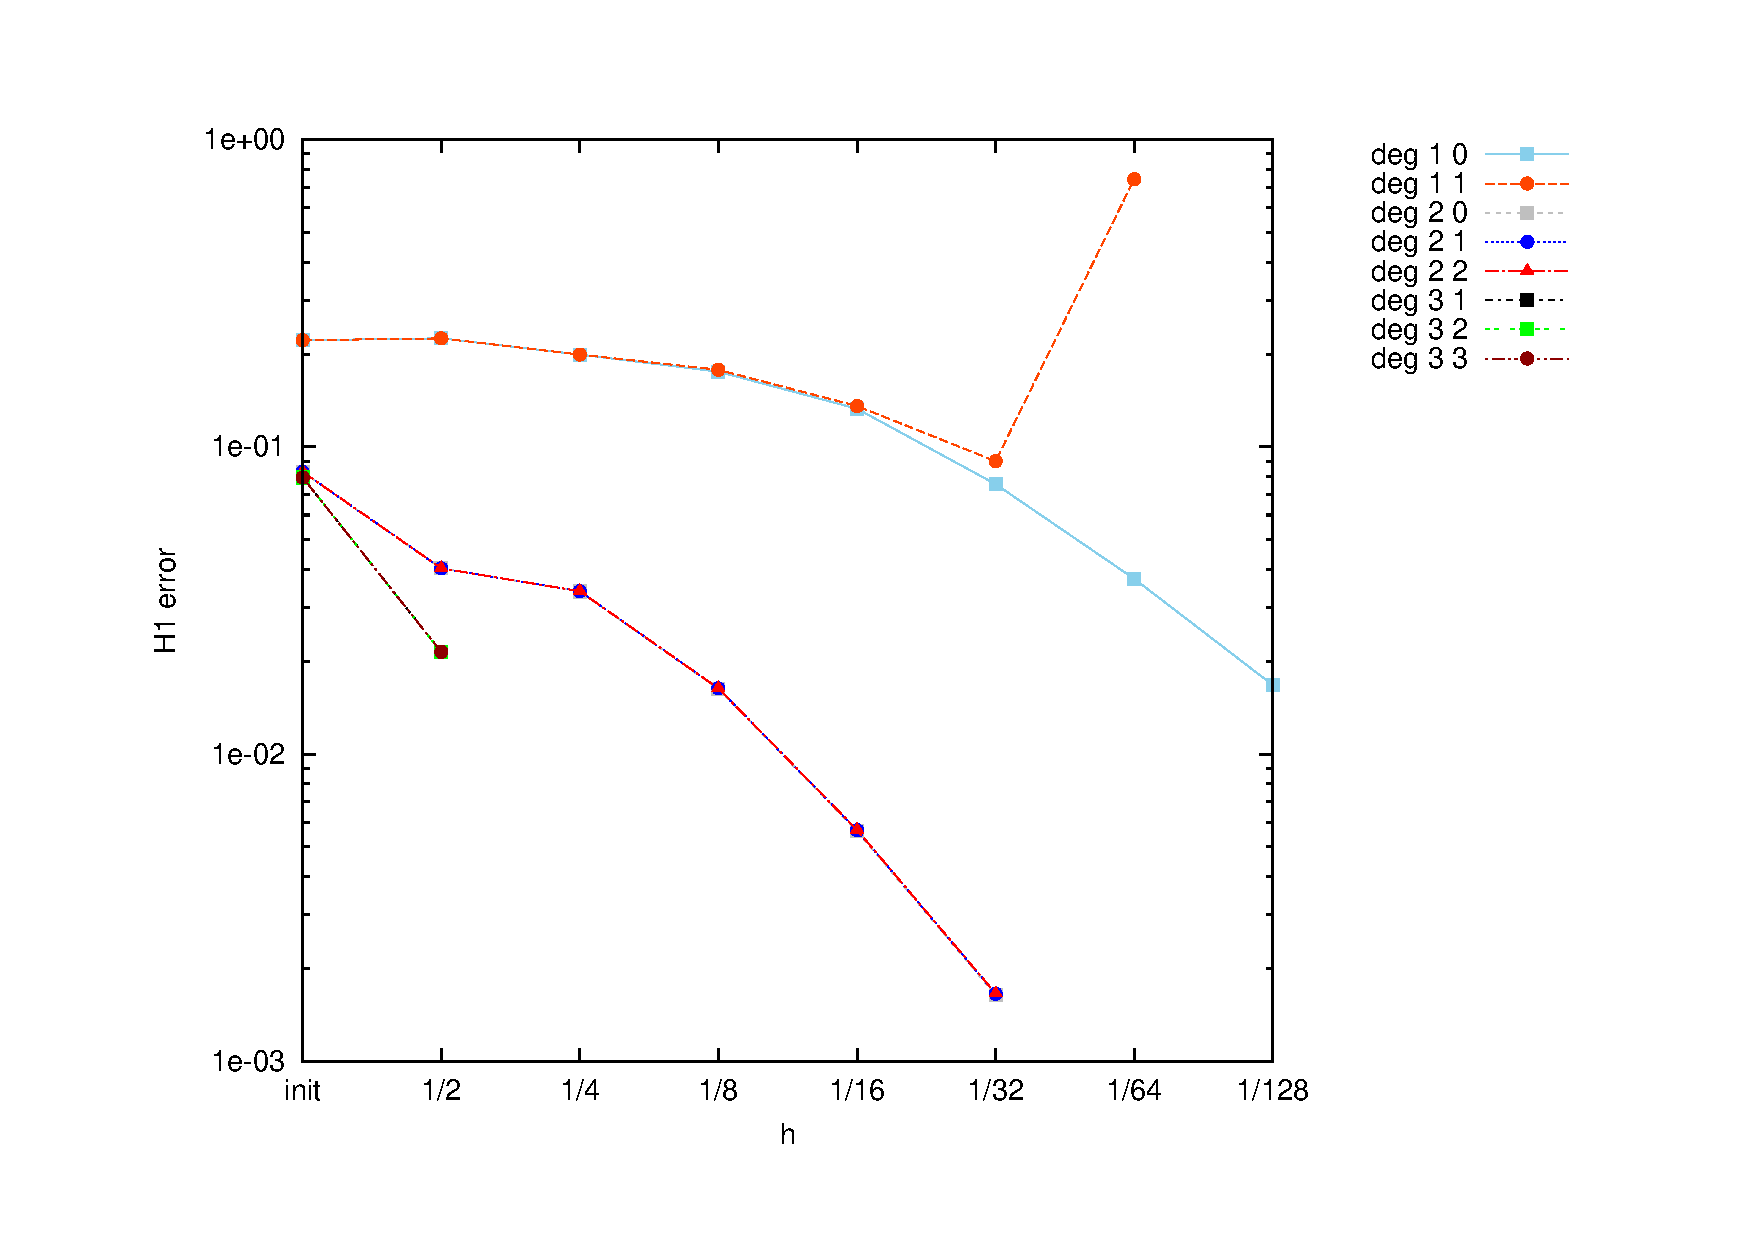
\includegraphics[scale =0.4]{../../FEniCS/diagrams/MA3_Neilan_GradJump_h1.pdf}
	\caption{$H^1$ errors for test case \ref{test singularity} and additional gradient jump penalty}
	\label{fig: h1 errors test 3 jump}
\end{figure}

\begin{table}[H]
\centering
\begin{subtable}[b]{0.45\textwidth}
	\pgfplotstabletypeset
	{
		k $k_{DH}$ {numerical order}
		1 0 0.8565
		2 1 1.32222
		2 2 1.32048
	}
	\caption{numerical order in $L2$ norm}
	\end{subtable}
	\begin{subtable}[b]{0.45\textwidth}
	\pgfplotstabletypeset
	{
		k $k_{DH}$ {numerical order}
		1 0 0.618481
		2 1 1.17823
		2 2 1.17823
	}
	\caption{numerical order in $H1$ norm}
	\end{subtable}
	\caption{numerical order with jump penalty in test \ref{test singularity}}
\label{tab: order jump 3}
\end{table}

